\documentclass[12pt,a4paper]{article}
\usepackage[utf8]{inputenc}
\usepackage[margin=1in]{geometry}
\usepackage{amsmath,amssymb,amsfonts}
\usepackage{graphicx}
\usepackage{xcolor}
\usepackage{listings}
\usepackage{tikz}
\usepackage{fancyhdr}
\usepackage{hyperref}
\usepackage{tcolorbox}
\usepackage{enumitem}
\usepackage{mdframed}
\usepackage{multicol}
\usepackage{float}

% TikZ libraries
\usetikzlibrary{shapes,arrows,positioning,automata,decorations.pathreplacing}

% Color definitions
\definecolor{codegreen}{rgb}{0,0.6,0}
\definecolor{codegray}{rgb}{0.5,0.5,0.5}
\definecolor{codepurple}{rgb}{0.58,0,0.82}
\definecolor{backcolour}{rgb}{0.95,0.95,0.92}
\definecolor{keywordcolor}{rgb}{0.0,0.0,1.0}
\definecolor{stringcolor}{rgb}{0.8,0.0,0.0}

% Code listing style
\lstdefinestyle{mystyle}{
    backgroundcolor=\color{backcolour},   
    commentstyle=\color{codegreen},
    keywordstyle=\color{keywordcolor},
    numberstyle=\tiny\color{codegray},
    stringstyle=\color{stringcolor},
    basicstyle=\ttfamily\footnotesize,
    breakatwhitespace=false,         
    breaklines=true,                 
    captionpos=b,                    
    keepspaces=true,                 
    numbers=left,                    
    numbersep=5pt,                  
    showspaces=false,                
    showstringspaces=false,
    showtabs=false,                  
    tabsize=2
}
\lstset{style=mystyle}

% Custom boxes
\newtcolorbox{definitionbox}[1]{
    colback=blue!5!white,
    colframe=blue!75!black,
    fonttitle=\bfseries,
    title=#1
}

\newtcolorbox{examplebox}[1]{
    colback=green!5!white,
    colframe=green!75!black,
    fonttitle=\bfseries,
    title=#1
}

\newtcolorbox{warningbox}[1]{
    colback=red!5!white,
    colframe=red!75!black,
    fonttitle=\bfseries,
    title=#1
}

\newtcolorbox{interactivebox}[1]{
    colback=orange!5!white,
    colframe=orange!75!black,
    fonttitle=\bfseries,
    title=#1
}

% Header and footer
\pagestyle{fancy}
\fancyhf{}
\fancyhead[L]{Circuit Breaker Pattern}
\fancyhead[R]{Distributed Systems}
\fancyfoot[C]{\thepage}

% Title page information
\title{\Huge \textbf{Circuit Breaker Pattern} \\
       \Large \textit{A Comprehensive Study for Distributed Systems} \\
       \vspace{0.5cm}
       \normalsize Professional Study Notes}
\author{Distributed Systems Engineering}
\date{June 2025}

\begin{document}

\maketitle
\newpage

\tableofcontents
\newpage

% ============================================================================
\section{Introduction and Motivation}
% ============================================================================

\subsection{The Problem: Cascading Failures in Distributed Systems}

In modern distributed architectures, services depend on multiple external components—databases, APIs, microservices, and third-party integrations. When one component fails, it can trigger a catastrophic chain reaction known as \textbf{cascading failure}.

\begin{definitionbox}{Cascading Failure}
A cascading failure occurs when the failure of a part of a system triggers the failure of successive parts, eventually leading to the failure of the entire system.
\end{definitionbox}

\subsubsection{Real-World Scenario: E-commerce Platform Meltdown}

Consider an e-commerce platform during Black Friday:

\begin{enumerate}
    \item Payment service becomes overloaded (high traffic)
    \item Order service starts timing out waiting for payment confirmation
    \item Order service threads become exhausted
    \item User interface becomes unresponsive
    \item Users refresh frantically, increasing load
    \item Entire platform crashes
\end{enumerate}

\begin{warningbox}{Critical Insight}
Without proper protection mechanisms, a single slow dependency can bring down your entire system, even if all other components are healthy.
\end{warningbox}

% ============================================================================
\section{Circuit Breaker Pattern: The Solution}
% ============================================================================

\subsection{Pattern Definition}

\begin{definitionbox}{Circuit Breaker Pattern}
The Circuit Breaker pattern prevents an application from repeatedly trying to execute an operation that's likely to fail, allowing it to detect when the fault has been resolved and resume normal operation.
\end{definitionbox}

\subsection{Electrical Circuit Analogy}

Just like electrical circuit breakers protect electrical systems from damage due to excess current, software circuit breakers protect distributed systems from cascading failures.

\begin{figure}[H]
\centering
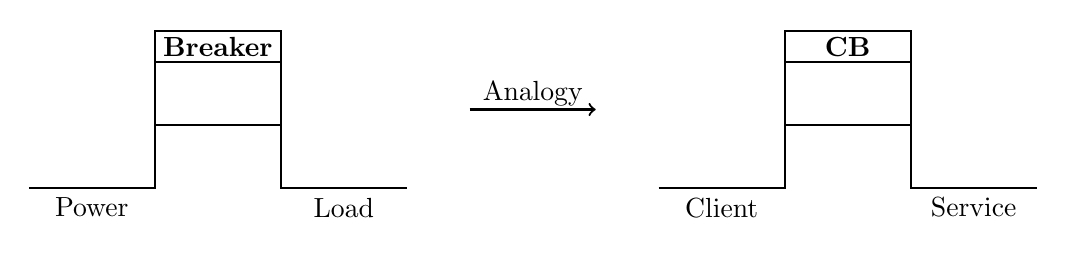
\begin{tikzpicture}[scale=0.8]
    % Electrical circuit
    \draw[thick] (0,0) -- (2,0) -- (2,1) -- (4,1) -- (4,0) -- (6,0);
    \draw[thick] (2,1) -- (2,2) rectangle (4,2.5);
    \draw[thick] (4,2.5) -- (4,2) -- (4,1);
    \node at (3,2.25) {\textbf{Breaker}};
    \node at (1,0) [below] {Power};
    \node at (5,0) [below] {Load};
    
    % Arrow
    \draw[thick, ->] (7,1.25) -- (9,1.25);
    \node at (8,1.5) {Analogy};
    
    % Software circuit
    \draw[thick] (10,0) -- (12,0) -- (12,1) -- (14,1) -- (14,0) -- (16,0);
    \draw[thick] (12,1) -- (12,2) rectangle (14,2.5);
    \draw[thick] (14,2.5) -- (14,2) -- (14,1);
    \node at (13,2.25) {\textbf{CB}};
    \node at (11,0) [below] {Client};
    \node at (15,0) [below] {Service};
\end{tikzpicture}
\caption{Circuit Breaker Analogy: Electrical vs Software}
\end{figure}

% ============================================================================
\section{Circuit Breaker States and Behavior}
% ============================================================================

\subsection{State Machine}

The circuit breaker operates as a finite state machine with three primary states:

\begin{figure}[H]
\centering
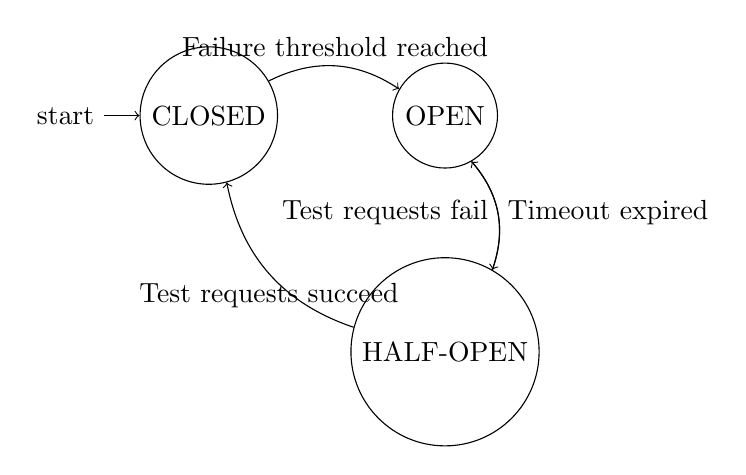
\begin{tikzpicture}[node distance=3cm, auto]
    % States
    \node[state, initial] (closed) {CLOSED};
    \node[state, right of=closed] (open) {OPEN};
    \node[state, below of=open] (halfopen) {HALF-OPEN};
    
    % Transitions
    \path[->] 
        (closed) edge[bend left] node[above] {Failure threshold reached} (open)
        (open) edge[bend left] node[right] {Timeout expired} (halfopen)
        (halfopen) edge[bend left] node[below] {Test requests succeed} (closed)
        (halfopen) edge[bend right] node[left] {Test requests fail} (open);
\end{tikzpicture}
\caption{Circuit Breaker State Machine}
\end{figure}

\subsection{State Descriptions}

\begin{definitionbox}{CLOSED State}
\textbf{Normal Operation:} All requests pass through to the service. Failures are counted, and if they exceed the threshold within a time window, the circuit opens.
\end{definitionbox}

\begin{definitionbox}{OPEN State}
\textbf{Fail-Fast Mode:} Requests immediately fail without calling the service. This prevents resource exhaustion and gives the failing service time to recover.
\end{definitionbox}

\begin{definitionbox}{HALF-OPEN State}
\textbf{Recovery Testing:} A limited number of requests are allowed through to test if the service has recovered. Success closes the circuit; failure reopens it.
\end{definitionbox}

\begin{interactivebox}{Quick Check}
\textbf{Question:} In which state does the circuit breaker provide the fastest response time for failed requests?

\textit{Answer: OPEN state - requests fail immediately without network calls.}
\end{interactivebox}

% ============================================================================
\section{Case Study: Netflix and the Need for Circuit Breakers}
% ============================================================================

\subsection{The Netflix Incident (2008)}

\subsubsection{Background}
Netflix's streaming service was experiencing intermittent issues with their recommendation service. The recommendation API was becoming slow and unreliable due to increased load.

\subsubsection{The Problem}
\begin{enumerate}
    \item Recommendation service started responding slowly (5-10 seconds)
    \item Video streaming service waited for recommendations before displaying content
    \item User threads in the streaming service became exhausted
    \item Entire video streaming became unavailable
    \item Customer satisfaction plummeted
\end{enumerate}

\subsubsection{Traditional Approach vs Circuit Breaker}

\begin{multicols}{2}
\textbf{Without Circuit Breaker:}
\begin{itemize}
    \item Keep retrying slow service
    \item Exhaust connection pools
    \item Block user threads
    \item System-wide failure
\end{itemize}

\columnbreak

\textbf{With Circuit Breaker:}
\begin{itemize}
    \item Detect recommendation failures
    \item Fail fast on subsequent calls
    \item Show content without recommendations
    \item Graceful degradation
\end{itemize}
\end{multicols}

\subsubsection{Solution Implementation}

Netflix implemented the circuit breaker pattern as part of their Hystrix library:

\begin{lstlisting}[language=Java, caption=Netflix Hystrix Example]
@HystrixCommand(fallbackMethod = "getDefaultRecommendations")
public List<Movie> getRecommendations(String userId) {
    return recommendationService.getRecommendations(userId);
}

public List<Movie> getDefaultRecommendations(String userId) {
    // Return popular movies or user's watch history
    return popularMoviesService.getTopMovies();
}
\end{lstlisting}

\subsubsection{Results}
\begin{itemize}
    \item \textbf{99.5\%} uptime improvement for video streaming
    \item \textbf{60\%} reduction in customer complaints
    \item Graceful degradation instead of complete failures
    \item Better user experience during service issues
\end{itemize}

% ============================================================================
\section{Implementation Strategies and Patterns}
% ============================================================================

\subsection{Key Configuration Parameters}

\begin{table}[H]
\centering
\begin{tabular}{|l|l|p{6cm}|}
\hline
\textbf{Parameter} & \textbf{Typical Value} & \textbf{Description} \\
\hline
Failure Threshold & 5-10 failures & Number of consecutive failures to open circuit \\
\hline
Timeout & 30-60 seconds & Time to wait before trying HALF-OPEN \\
\hline
Success Threshold & 3-5 successes & Successes needed in HALF-OPEN to close \\
\hline
Failure Rate & 50-70\% & Percentage failure rate to open circuit \\
\hline
Request Volume & 10-20 requests & Minimum requests before considering failure rate \\
\hline
\end{tabular}
\caption{Circuit Breaker Configuration Parameters}
\end{table}

\subsection{Implementation Patterns}

\subsubsection{1. Count-Based Circuit Breaker}
Opens after a specific number of consecutive failures.

\begin{lstlisting}[language=Go, caption=Count-Based Circuit Breaker Logic]
type CountBasedCircuitBreaker struct {
    consecutiveFailures int
    failureThreshold   int
    state             State
}

func (cb *CountBasedCircuitBreaker) Execute(fn func() error) error {
    if cb.state == OPEN {
        return ErrCircuitOpen
    }
    
    err := fn()
    if err != nil {
        cb.consecutiveFailures++
        if cb.consecutiveFailures >= cb.failureThreshold {
            cb.state = OPEN
        }
        return err
    }
    
    cb.consecutiveFailures = 0
    return nil
}
\end{lstlisting}

\subsubsection{2. Time-Window Circuit Breaker}
Considers failure rate within a sliding time window.

\begin{lstlisting}[language=Go, caption=Time-Window Circuit Breaker Logic]
type TimeWindowCircuitBreaker struct {
    failures      []time.Time
    requests      []time.Time
    windowSize    time.Duration
    failureRate   float64
    minRequests   int
}

func (cb *TimeWindowCircuitBreaker) shouldOpen() bool {
    now := time.Now()
    // Clean old entries
    cb.cleanOldEntries(now)
    
    if len(cb.requests) < cb.minRequests {
        return false
    }
    
    currentFailureRate := float64(len(cb.failures)) / float64(len(cb.requests))
    return currentFailureRate >= cb.failureRate
}
\end{lstlisting}

% ============================================================================
\section{Advanced Topics and Best Practices}
% ============================================================================

\subsection{Fallback Strategies}

\begin{examplebox}{Fallback Patterns}
\begin{enumerate}
    \item \textbf{Default Response:} Return cached or default data
    \item \textbf{Alternative Service:} Route to backup service
    \item \textbf{Graceful Degradation:} Reduce functionality
    \item \textbf{Queue for Later:} Store requests for later processing
\end{enumerate}
\end{examplebox}

\subsection{Monitoring and Observability}

\subsubsection{Key Metrics to Track}

\begin{table}[H]
\centering
\begin{tabular}{|l|l|}
\hline
\textbf{Metric} & \textbf{Purpose} \\
\hline
Request Count & Total requests processed \\
\hline
Failure Count & Number of failed requests \\
\hline
Success Rate & Percentage of successful requests \\
\hline
State Changes & Frequency of state transitions \\
\hline
Response Time & Service response time distribution \\
\hline
Circuit Open Duration & Time spent in OPEN state \\
\hline
\end{tabular}
\caption{Circuit Breaker Monitoring Metrics}
\end{table}

\subsection{Anti-Patterns and Common Mistakes}

\begin{warningbox}{Common Anti-Patterns}
\begin{enumerate}
    \item \textbf{Too Aggressive Thresholds:} Opening circuit too quickly
    \item \textbf{No Fallback:} Failing without graceful degradation
    \item \textbf{Synchronous Fallbacks:} Fallback calls that can also fail
    \item \textbf{Ignoring Half-Open:} Not properly testing recovery
    \item \textbf{Circuit Per Instance:} Not sharing state across instances
\end{enumerate}
\end{warningbox}

% ============================================================================
\section{Project Example: Financial Trading Platform}
% ============================================================================

\subsection{System Architecture}

Our implementation demonstrates circuit breakers in a financial trading platform with the following components:

\begin{figure}[H]
\centering
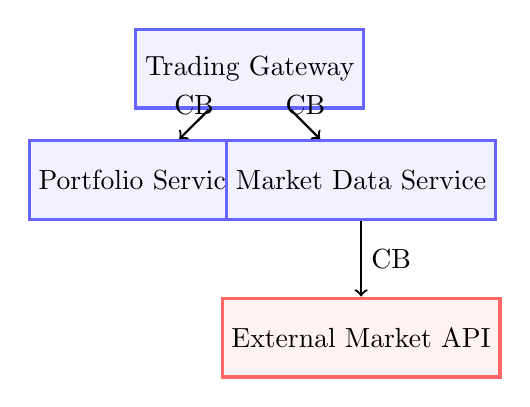
\begin{tikzpicture}[
    node distance=2cm,
    service/.style={rectangle, draw=blue!60, fill=blue!5, very thick, minimum size=1cm},
    database/.style={cylinder, draw=green!60, fill=green!5, very thick, minimum size=1cm},
    external/.style={rectangle, draw=red!60, fill=red!5, very thick, minimum size=1cm}
]
    % Services
    \node[service] (gateway) {Trading Gateway};
    \node[service, below left of=gateway] (portfolio) {Portfolio Service};
    \node[service, below right of=gateway] (market) {Market Data Service};
    \node[external, below of=market] (external_api) {External Market API};
    
    % Arrows with circuit breakers
    \draw[thick, ->] (gateway) -- (portfolio) node[midway, above] {CB};
    \draw[thick, ->] (gateway) -- (market) node[midway, above] {CB};
    \draw[thick, ->] (market) -- (external_api) node[midway, right] {CB};
\end{tikzpicture}
\caption{Trading Platform with Circuit Breakers}
\end{figure}

\subsection{Failure Scenarios and Protection}

\subsubsection{Scenario 1: Market Data Service Overload}

\begin{examplebox}{Market Data Failure Scenario}
\textbf{Problem:} External market data provider becomes slow during market volatility.

\textbf{Without Circuit Breaker:}
\begin{itemize}
    \item Trading gateway waits 30+ seconds for market data
    \item User threads become exhausted
    \item All trading requests fail
    \item System becomes completely unavailable
\end{itemize}

\textbf{With Circuit Breaker:}
\begin{itemize}
    \item Circuit breaker detects market data failures
    \item Subsequent requests fail fast (< 1ms)
    \item Fallback returns cached prices
    \item Trading continues with slightly stale data
    \item System remains responsive
\end{itemize}
\end{examplebox}

\subsubsection{Implementation Example}

\begin{lstlisting}[language=Go, caption=Trading Gateway with Circuit Breaker]
type TradingGateway struct {
    marketDataCB   *circuitbreaker.CircuitBreaker
    portfolioCB    *circuitbreaker.CircuitBreaker
    priceCache     *PriceCache
}

func (tg *TradingGateway) ExecuteTrade(trade TradeRequest) (*TradeResponse, error) {
    // Get current price with circuit breaker protection
    price, err := tg.marketDataCB.Execute(func() (interface{}, error) {
        return tg.getMarketPrice(trade.Symbol)
    })
    
    if err != nil {
        // Fallback to cached price
        if cachedPrice := tg.priceCache.Get(trade.Symbol); cachedPrice != nil {
            price = cachedPrice
        } else {
            return nil, fmt.Errorf("market data unavailable")
        }
    }
    
    // Execute trade with portfolio service
    result, err := tg.portfolioCB.Execute(func() (interface{}, error) {
        return tg.executeWithPortfolio(trade, price)
    })
    
    if err != nil {
        // Fallback: queue trade for later execution
        tg.queueTradeForLater(trade)
        return &TradeResponse{
            Status: "QUEUED",
            Message: "Trade queued due to system issues",
        }, nil
    }
    
    return result.(*TradeResponse), nil
}
\end{lstlisting}

% ============================================================================
\section{Testing and Validation}
% ============================================================================

\subsection{Testing Circuit Breaker Behavior}

\begin{interactivebox}{Testing Checklist}
Test each state transition:
\begin{enumerate}
    \item \textbf{CLOSED → OPEN:} Verify threshold triggers opening
    \item \textbf{OPEN → HALF-OPEN:} Confirm timeout triggers recovery attempt
    \item \textbf{HALF-OPEN → CLOSED:} Success threshold closes circuit
    \item \textbf{HALF-OPEN → OPEN:} Any failure reopens circuit
\end{enumerate}
\end{interactivebox}

\subsection{Load Testing Example}

\begin{lstlisting}[language=bash, caption=Circuit Breaker Load Test]
#!/bin/bash
# Simulate high load and service failures

echo "Phase 1: Normal operation"
for i in {1..20}; do
    curl -X POST http://localhost:8080/api/v1/trades \
         -H "Content-Type: application/json" \
         -d '{"userId":"user'$i'","symbol":"AAPL","quantity":10}'
    sleep 0.1
done

echo "Phase 2: Introduce failures"
# Make market data service fail 80% of requests
curl -X POST http://localhost:8082/api/v1/simulate/failure \
     -d '{"failure_rate": 0.8}'

echo "Phase 3: Trigger circuit breaker"
for i in {1..10}; do
    curl -X POST http://localhost:8080/api/v1/trades \
         -H "Content-Type: application/json" \
         -d '{"userId":"user'$i'","symbol":"AAPL","quantity":1}'
done

echo "Phase 4: Verify fast failures"
# Check that requests now fail quickly
curl http://localhost:8080/api/v1/circuit-breaker/status
\end{lstlisting}

% ============================================================================
\section{Metrics and Monitoring}
% ============================================================================

\subsection{Prometheus Metrics}

Our implementation exposes comprehensive metrics:

\begin{lstlisting}[language=Go, caption=Circuit Breaker Metrics]
var (
    requestsTotal = prometheus.NewCounterVec(
        prometheus.CounterOpts{
            Name: "circuit_breaker_requests_total",
            Help: "Total number of requests processed by circuit breaker",
        },
        []string{"circuit_name", "state", "result"},
    )
    
    stateChanges = prometheus.NewCounterVec(
        prometheus.CounterOpts{
            Name: "circuit_breaker_state_changes_total",
            Help: "Total number of state changes",
        },
        []string{"circuit_name", "from_state", "to_state"},
    )
    
    currentState = prometheus.NewGaugeVec(
        prometheus.GaugeOpts{
            Name: "circuit_breaker_state",
            Help: "Current state of the circuit breaker (0=CLOSED, 1=OPEN, 2=HALF_OPEN)",
        },
        []string{"circuit_name"},
    )
)
\end{lstlisting}

\subsection{Alerting Rules}

\begin{lstlisting}[language=yaml, caption=Prometheus Alerting Rules]
groups:
- name: circuit_breaker_alerts
  rules:
  - alert: CircuitBreakerOpen
    expr: circuit_breaker_state > 0
    for: 5m
    labels:
      severity: warning
    annotations:
      summary: "Circuit breaker {{ $labels.circuit_name }} is open"
      description: "Circuit breaker has been open for more than 5 minutes"
      
  - alert: HighFailureRate
    expr: |
      (
        rate(circuit_breaker_requests_total{result="failure"}[5m]) /
        rate(circuit_breaker_requests_total[5m])
      ) > 0.5
    for: 2m
    labels:
      severity: critical
    annotations:
      summary: "High failure rate detected"
      description: "Failure rate is above 50% for 2 minutes"
\end{lstlisting}

% ============================================================================
\section{Performance Analysis}
% ============================================================================

\subsection{Latency Comparison}

\begin{table}[H]
\centering
\begin{tabular}{|l|c|c|c|}
\hline
\textbf{Scenario} & \textbf{Without CB} & \textbf{With CB (Closed)} & \textbf{With CB (Open)} \\
\hline
Normal Operation & 50ms & 52ms & N/A \\
\hline
Service Slow (5s) & 5000ms & 5000ms & 1ms \\
\hline
Service Down & 30000ms (timeout) & 30000ms & 1ms \\
\hline
Recovery Time & 10+ minutes & 10+ minutes & 30 seconds \\
\hline
\end{tabular}
\caption{Performance Impact of Circuit Breaker}
\end{table}

\subsection{Resource Utilization}

\begin{examplebox}{Resource Impact Analysis}
\begin{itemize}
    \item \textbf{CPU Overhead:} < 0.1\% for circuit breaker logic
    \item \textbf{Memory:} ~1KB per circuit breaker instance
    \item \textbf{Network:} No additional network calls
    \item \textbf{Thread Pool:} Prevents thread exhaustion
\end{itemize}
\end{examplebox}

% ============================================================================
\section{Future Considerations and Extensions}
% ============================================================================

\subsection{Advanced Patterns}

\subsubsection{Bulkhead Pattern Integration}
Combine circuit breakers with bulkhead pattern for complete isolation:

\begin{lstlisting}[language=Go, caption=Bulkhead + Circuit Breaker]
type ServiceClient struct {
    circuitBreaker *CircuitBreaker
    threadPool     *ThreadPool
    semaphore      *Semaphore
}

func (sc *ServiceClient) Call(request Request) (*Response, error) {
    // Acquire semaphore (bulkhead)
    if !sc.semaphore.TryAcquire() {
        return nil, ErrResourceExhausted
    }
    defer sc.semaphore.Release()
    
    // Execute with circuit breaker
    return sc.circuitBreaker.Execute(func() (*Response, error) {
        return sc.makeAPICall(request)
    })
}
\end{lstlisting}

\subsection{Machine Learning Integration}

Future enhancements could include:
\begin{itemize}
    \item \textbf{Adaptive Thresholds:} ML-based threshold adjustment
    \item \textbf{Predictive Opening:} Open circuit before failures occur
    \item \textbf{Pattern Recognition:} Identify failure patterns
    \item \textbf{Anomaly Detection:} Detect unusual service behavior
\end{itemize}

% ============================================================================
\section{Summary and Key Takeaways}
% ============================================================================

\begin{interactivebox}{Revision Summary}
\textbf{Key Concepts to Remember:}
\begin{enumerate}
    \item Circuit breakers prevent cascading failures in distributed systems
    \item Three states: CLOSED (normal), OPEN (failing), HALF-OPEN (testing)
    \item Essential for any system with external dependencies
    \item Must be combined with fallback strategies
    \item Proper monitoring and alerting are crucial
\end{enumerate}

\textbf{When to Use Circuit Breakers:}
\begin{itemize}
    \item Remote service calls (HTTP APIs, databases, message queues)
    \item Any operation that can fail or timeout
    \item Systems requiring high availability
    \item Microservices architectures
\end{itemize}

\textbf{Common Failure Modes to Avoid:}
\begin{itemize}
    \item No fallback strategy
    \item Thresholds too aggressive or too lenient
    \item Not monitoring circuit breaker metrics
    \item Sharing circuit breakers across unrelated operations
\end{itemize}
\end{interactivebox}

% ============================================================================
\section{Hands-On Exercises}
% ============================================================================

\begin{interactivebox}{Exercise 1: State Machine Analysis}
Given a circuit breaker with the following configuration:
\begin{itemize}
    \item Failure threshold: 5 failures
    \item Timeout: 30 seconds
    \item Success threshold: 3 successes
\end{itemize}

Trace through the following sequence of requests and determine the final state:
\begin{enumerate}
    \item 3 successful requests
    \item 6 consecutive failures
    \item Wait 35 seconds
    \item 2 successful requests
    \item 1 failure
    \item 3 successful requests
\end{enumerate}

\textit{Solution: CLOSED → OPEN → HALF-OPEN → OPEN → HALF-OPEN → CLOSED}
\end{interactivebox}

\begin{interactivebox}{Exercise 2: Configuration Tuning}
You have a payment service that:
\begin{itemize}
    \item Normal response time: 200ms
    \item Timeout after: 5 seconds
    \item Fails 2\% of the time normally
    \item During incidents, fails 80\% with 10-second responses
\end{itemize}

Design appropriate circuit breaker parameters and justify your choices.

\textit{Consider: failure threshold, timeout, failure rate threshold, minimum requests}
\end{interactivebox}

% ============================================================================
\section{References and Further Reading}
% ============================================================================

\begin{enumerate}
    \item Fowler, Martin. "CircuitBreaker." Martin Fowler's Blog, 2014.
    \item Nygard, Michael T. "Release It! Design and Deploy Production-Ready Software." 2nd ed., 2018.
    \item Netflix Technology Blog. "Introducing Hystrix for Resilience Engineering." 2012.
    \item Tanenbaum, Andrew S., and Maarten van Steen. "Distributed Systems: Principles and Paradigms." 3rd ed., 2017.
    \item Kleppmann, Martin. "Designing Data-Intensive Applications." O'Reilly Media, 2017.
    \item Richardson, Chris. "Microservices Patterns." Manning Publications, 2018.
\end{enumerate}

\vspace{1cm}

\begin{center}
\textit{End of Study Notes}

\textit{For practical implementation, refer to the accompanying Go project demonstrating a production-ready circuit breaker in a financial trading platform.}
\end{center}

\end{document}
